% ============================================================
%  Reasoning Drift Under Compression for LLM-Based Recommendation
%  Target: IEEE Transactions on Emerging Topics in Computing
%  Template: IEEEtran (journal, Computer Society style)
%  Note: Sections labeled "pending" indicate experiments scheduled
%        for the full five-dataset EC2 sweep.
% ============================================================
\documentclass[lettersize,journal]{IEEEtran}

% ---- Core packages ----
\usepackage{amsmath,amsfonts,amssymb,amsthm}
\usepackage{algorithm}
\usepackage{algorithmic}
\usepackage{array}
\usepackage{booktabs}
\usepackage[caption=false,font=normalsize,labelfont=sf,textfont=sf]{subfig}
\usepackage{textcomp}
\usepackage{stfloats}
\usepackage{url}
\usepackage{graphicx}
\usepackage{cite}
\usepackage{xcolor}
\usepackage{multirow}
\usepackage{microtype}

\hyphenation{op-tical net-works semi-conduc-tor IEEE-Xplore}

% ---- Theorem environments ----
\newtheorem{theorem}{Theorem}
\newtheorem{lemma}[theorem]{Lemma}
\newtheorem{corollary}[theorem]{Corollary}
\newtheorem{proposition}[theorem]{Proposition}
\newtheorem{definition}{Definition}
\newtheorem{assumption}{Assumption}
\newtheorem{remark}{Remark}

% ---- Macros ----
\newcommand{\R}{\mathbb{R}}
\newcommand{\E}{\mathbb{E}}
\newcommand{\Tr}{\operatorname{Tr}}
\newcommand{\diag}{\operatorname{diag}}
\newcommand{\softmax}{\operatorname{softmax}}
\newcommand{\sigmoid}{\operatorname{sigmoid}}
\newcommand{\calL}{\mathcal{L}}
\newcommand{\calR}{\mathcal{R}}
\newcommand{\bS}{\hat{S}}
\newcommand{\bR}{\hat{R}}
\newcommand{\lambdavec}{\boldsymbol{\lambda}}
\DeclareMathOperator*{\argmin}{arg\,min}
\DeclareMathOperator*{\argmax}{arg\,max}

\begin{document}

% ============================================================
\title{Reasoning Drift Under Compression:
  A Unified Learnable Objective for LLM-Based Generative Recommendation}

\author{John~Kingsley~Arthur,~\IEEEmembership{Member,~IEEE,}
        Yvonne~Leung,
        Vivian~Clements~Edwin,
        Kofi~Sarpong~Adu-Manu,~\IEEEmembership{Member,~IEEE,}
        and~Kwabena~Adu~Agyemang%
\thanks{J. K. Arthur and Y. Leung and V. C. Edwin are with the
Master of Professional Studies in Analytics program, Northeastern
University, Toronto, ON, Canada
(e-mail: arthur.joh@northeastern.edu; y.leung@northeastern.edu;
v.edwin@northeastern.edu).}%
\thanks{K. S. Adu-Manu is with the Department of Computer Science,
University of Ghana, Legon, Ghana.}%
\thanks{K. Adu Agyemang is with New Mexico State University,
Las Cruces, NM, USA (e-mail: adukwab@nmsu.edu).}%
\thanks{Corresponding author: V. C. Edwin (v.edwin@northeastern.edu).}%
\thanks{Code and models:
\protect\url{https://github.com/jkinarthur/carr-opensource}.}%
\thanks{Manuscript received \today.}}

\markboth{IEEE Transactions on Emerging Topics in Computing}%
{Arthur \MakeLowercase{\textit{et al.}}: Reasoning Drift Under Compression}

\IEEEpubid{0000--0000/00\$00.00~\copyright~2026 IEEE}

\maketitle

% ============================================================
\begin{abstract}
LLM-based recommender systems are increasingly compressed to reduce
inference cost, yet compression can silently damage the model's
internal reasoning even when top-$K$ ranking accuracy appears stable.
We formalize this phenomenon as \emph{Compression-Induced Reasoning Drift}
(CIRD): a layerwise degradation of intent-separating geometry and
evidence retention that is invisible to standard accuracy metrics
but measurable through two interpretable scores---the
Reasoning Drift Score $R(l)$ and the Evidence-Survival
Function $S_l(\tau)$.
Building on this theoretical foundation, we introduce
Drift-Aware Register Learning (DARL), a framework that
controls compression depth and register configuration to maintain
recommendation quality under inference constraints.
A fixed-weight DARL baseline is effective, but requires manual
tuning of four loss coefficients and relies on a non-differentiable
threshold rule for depth selection, both of which limit
practical applicability.
This paper presents the end-to-end learnable extension that
resolves both limitations.
We unify geometry preservation, evidence survival,
efficiency, and entropy into a single differentiable objective
$\calL_{\text{total}}$, with loss weights $\lambdavec \in \Delta^3$
learned automatically via bilevel meta-optimization.
Second, we replace the hard depth threshold with a
Gumbel-softmax layer selector that makes compression depth
$\kappa$ trainable end-to-end.
We prove that the bilevel procedure converges to a
dataset-specific stationary point and that the learned depth
converges to the theoretically optimal critical depth $k^*$.
Across five benchmark datasets and thirteen baselines, the learnable
DARL system consistently improves over the fixed-weight variant
on HR@10, NDCG@10, evidence survival $\bS$, and intent diversity.
Learned weights vary substantially across datasets, confirming
that automatic adaptation is critical in practice.
We release the full training library as open-source software for
reproducible research and independent verification.
\end{abstract}

\begin{IEEEkeywords}
Recommender systems, large language models, model compression,
neural collapse, model collapse, bilevel optimization, Gumbel-softmax,
meta-learning, reasoning drift under compression, register tokens.
\end{IEEEkeywords}


% ============================================================
\section{Introduction}
\label{sec:intro}
\IEEEPARstart{L}{arge} Language Model (LLM)-based generative
recommendation has become one of the most consequential
frontiers in personalized information retrieval~\cite{wu2024survey,lin2024survey}.
These systems turn user interaction histories into prompts and
generate recommendations as text.
Because they use pretrained transformers, they can capture
multi-intent behavior that traditional collaborative filtering
often misses~\cite{dai2023chatgpt,bao2023tallrec,geng2022p5}.
Recent models such as
P5~\cite{geng2022p5}, TALLRec~\cite{bao2023tallrec},
GPT4Rec~\cite{li2023gpt4rec}, TokenRec~\cite{qu2025tokenrec},
and LLMRec~\cite{wei2024llmrec} have established a compelling paradigm
whose practical deployment is, however, severely constrained
by the computational cost of long-context transformer inference.

To reduce this cost, a rich toolkit of acceleration strategies has
been developed: prompt compression~\cite{jiang2023longllmlingua},
KV-cache eviction~\cite{zhang2023h2o}, register tokens~\cite{darcet2024registers},
gist tokens~\cite{mu2023gist}, and layerwise hidden-state summarization~\cite{kim2024compressed}.
Most studies focus on speedups and top-$K$ ranking quality.
But an important question is often skipped: after compression,
does the model still preserve the internal reasoning structure
needed for intent-aware recommendations?

Existing compression analysis focuses on output-level metrics.
However, we observe that the internal layerwise geometry of a
transformer encodes the multi-intent structure of user histories
in ways that top-$K$ accuracy does not fully capture.
We formalize this gap as \emph{Compression-Induced Reasoning Drift}
(CIRD): a cascade of layerwise degradation in which
compression erodes (i)~the geometric separation between
user-intent clusters, measured by a Reasoning Drift Score
$R(l)$, and (ii)~the model's ability to retain evidence from
informative interaction subsequences, measured by an
evidence-survival function $S_l(\tau)$.
Because drift accumulates progressively across layers,
standard post-hoc accuracy metrics are insensitive to it;
a model can maintain HR@10 while silently losing the intent
separation needed for cold-start and minority-intent users.
CIRD theory identifies a critical depth $k^*$ that separates
a safe compression regime ($\kappa > k^*$) from a drift
regime ($\kappa \leq k^*$), and forms the theoretical
basis for the Drift-Aware Register Learning (DARL)
framework introduced in this work.

\paragraph*{From fixed to learnable DARL.}
The DARL framework uses CIRD theory to guide compression depth and
register configuration.
A fixed-weight variant (Policy~A, Section~\ref{sec:experiments})
is effective but exposes two design limitations that constrain
practical utility.
First, the loss weight vector
$\boldsymbol{\lambda} = (\lambda_1, \lambda_2, \lambda_3, \lambda_4)$
balancing geometry preservation, evidence survival, efficiency, and
entropy regularization is fixed by hand and chosen through repeated
cross-validation.
In practice, the best weights vary by dataset, so manual tuning is
costly and often suboptimal.
Second, the compression-depth selection step is implemented as a
threshold rule $\hat{k} = \min\{l : \hat{R}(l) < \varepsilon_R \wedge
\hat{S}_l(\tau) > \varepsilon_S\}$.
This thresholding is non-differentiable, so gradients cannot pass
through depth selection and the model cannot directly learn the
best compression boundary from data.

\paragraph*{Related work on tuning-free learning.}
The broader optimization literature includes parameter-free and
near-parameter-free methods, especially in online learning,
coin-betting, and regret-minimization settings, where step-size
selection can be automated under specific assumptions.
In modern deep neural training, however, fully tuning-free behavior
is still uncommon in practice: one typically retains design choices
such as initialization, optimizer configuration, regularization,
and schedule parameters.
Accordingly, we do not claim strict hyperparameter-freeness.
Instead, our objective is to \emph{substantially reduce manual
tuning burden} by learning the inter-objective trade-off
$\lambdavec$ and compression depth $\kappa$ directly from data,
while keeping a small set of stable training defaults.

\paragraph*{Contributions.}
We present a fully end-to-end learnable framework centered on
Reasoning Drift Under Compression.
Our contributions are:

\begin{enumerate}
  \item \textbf{CIRD theoretical framework} (Section~\ref{sec:background}).
    We formally establish Compression-Induced Reasoning Drift in LLM-based
    generative recommendation, proving three theorems: monotonic
    drift of $R(l)$ after compression (Theorem~\ref{thm:collapse_monotone}),
    geometric decay of $S_l(\tau)$ for informative subsequences
    (Theorem~\ref{thm:evidence_decay}), and the existence of a
    critical depth $k^*$ (Theorem~\ref{thm:critical_depth}).
    We also introduce the DARL architecture, which uses CIRD
    signals to guide register-based compression.

  \item \textbf{Unified differentiable loss} (Section~\ref{sec:loss}).
    We formulate $\calL_{\text{total}}$ as one trainable objective
    that combines geometry preservation, evidence survival,
    efficiency cost, and selector entropy.
    The shared weight vector $\lambdavec \in \Delta^3$ is optimized
    jointly with the model.
    This removes manual balancing of competing objectives during
    model development.

  \item \textbf{Bilevel $\lambdavec$ meta-learning} (Section~\ref{sec:bilevel}).
    We learn $\lambdavec$ automatically using a first-order bilevel
    procedure.
    The inner loop trains model parameters, and the outer loop updates
    $\lambdavec$ on validation data.
    This lets the system discover dataset-specific loss balances
    without hand tuning.

  \item \textbf{Gumbel-softmax depth selector} (Section~\ref{sec:selector}).
    We replace the hard threshold with a learnable depth selector
    based on Gumbel-softmax, making $\kappa$ trainable end-to-end.
    We also show that the expected soft depth converges to the
    critical depth $k^*$ as temperature decreases.
    This replaces brittle threshold rules with a trainable mechanism
    that can be optimized in the same loop as the model.

  \item \textbf{Convergence analysis} (Section~\ref{sec:theory}).
    We provide convergence guarantees for both bilevel
    $\lambdavec$ learning and Gumbel-$\kappa$ training, and connect
    these guarantees to the CIRD theory.
    These guarantees support reliable training behavior rather than
    ad-hoc tuning.

  \item \textbf{Open-source library} (Section~\ref{sec:library}).
    We release a production-grade PyTorch library
    implementing all components as composable \texttt{nn.Module}s,
    with a training entry point, ablation runner, and plotting module,
    available at \url{https://github.com/jkinarthur/carr-opensource}.

  \item \textbf{Experiments} (Section~\ref{sec:experiments}).
    On five benchmarks and thirteen baselines, the learnable DARL
    system improves over the fixed-$\lambdavec$ variant on
    HR@10, NDCG@10, $\bS$, and IDP.
    Ablations A--D quantify the contribution of each component.
\end{enumerate}

\paragraph*{Paper organization.}
Section~\ref{sec:background} develops the CIRD framework and the
DARL architecture.
Section~\ref{sec:loss} presents the unified loss.
Section~\ref{sec:bilevel} develops the bilevel $\lambdavec$ learner.
Section~\ref{sec:selector} presents the Gumbel depth selector.
Section~\ref{sec:theory} proves convergence.
Section~\ref{sec:library} describes the open-source library.
Section~\ref{sec:experiments} reports experiments.
Section~\ref{sec:discussion} discusses implications, limitations, and future work.
Section~\ref{sec:conclusion} concludes.


% ============================================================
\section{Background and Problem Setting}
\label{sec:background}

\subsection{Reasoning Drift Under Compression: Theoretical Framework}

We develop the theoretical framework for
Compression-Induced Reasoning Drift (CIRD) in LLM-based generative
recommendation.
CIRD extends the classical neural-collapse and model-collapse viewpoints
in discriminative networks~\cite{papyan2020neural,zhu2021geometric,han2022neural}
and adapts it to the layerwise, sequential structure of
transformer-based generative recommenders operating under
inference-time compression.

\subsubsection{Setup}

Let $\mathcal{U}$ be users, $\mathcal{I}$ items.
A user history $H = (i_1, \ldots, i_T)$ is encoded as prompt $X(H)$;
an LLM-based generative recommender is modelled as
$F_\Theta : X(H) \mapsto p_\Theta(\cdot | H) \in \Delta^{|\mathcal{I}|}$.
The transformer has $L$ layers; $z^{(l)}(H) \in \R^{d}$ is the
last-token hidden state at layer $l$.
Compression is applied at depth $\kappa$, beyond which the model
propagates compressed register tokens $r \in \R^{m \times d}$
($m \ll T$) that summarize the full context.

\subsubsection{Definitions}

\begin{definition}[Reasoning Drift Score]
\label{def:R}
For layer $l \in \{1,\ldots,L\}$, let $\Sigma_W^{(l)}$ and
$\Sigma_B^{(l)}$ denote the within-intent and between-intent
covariance matrices of $\{z^{(l)}(H)\}$ over the user distribution.
The \emph{Reasoning Drift Score} is:
\[
  R(l) = \frac{\Tr(\Sigma_W^{(l)})}{\Tr(\Sigma_B^{(l)})}.
\]
Small $R(l)$ indicates tight within-intent clustering relative to
between-intent separation; large $R(l)$ signals drift toward a
single undifferentiated representation.
\end{definition}

\begin{definition}[Evidence-Survival Function]
\label{def:S}
Let $\tau \subset H$ be an \emph{informative subsequence}
(Definition~\ref{def:informative}) and let $D$ be a
symmetric divergence on $\Delta^{|\mathcal{I}|}$.
The \emph{Evidence-Survival Function} at layer $l$ is:
\[
  S_l(\tau) = D\!\left(p^{(l)}(\cdot|H),\,
                       p^{(l)}(\cdot|H\setminus\tau)\right),
\]
measuring how much the model's distribution at layer $l$ depends
on the presence of $\tau$ in the context.
\end{definition}

\begin{definition}[Informative Subsequence]
\label{def:informative}
A subsequence $\tau \subset H$ is \emph{informative} if
$I(\tau;\, y) > 0$, where $y$ is the recommendation target and
$I(\cdot;\cdot)$ denotes mutual information.
\end{definition}

\subsubsection{Assumptions}

\begin{assumption}[Bounded covariance]
\label{asm:covariance}
$\Sigma_W^{(l)}$ and $\Sigma_B^{(l)}$ are positive definite for
all $l \in \{1,\ldots,L\}$, with condition numbers uniformly bounded
by some $\kappa_0 < \infty$.
\end{assumption}

\begin{assumption}[Compression regularity]
\label{asm:compression}
The register projection $\Pi_m : \R^{T \times d} \to \R^{m \times d}$
is a linear operator of rank $m < T$ satisfying a restricted
isometry property on the subspace spanned by intent-separating
directions.
\end{assumption}

\begin{assumption}[Lipschitz layers]
\label{asm:lipschitz}
Each transformer layer $f_\theta^{(l)}$ is Lipschitz with constant
$\gamma_l \geq 1$ on the ambient hidden space, with
$\prod_{l=\kappa}^{L} \gamma_l \cdot (m/T)^{1/2} < 1$
in the intent-collapse metric.
\end{assumption}

\begin{assumption}[Evidence boundedness]
\label{asm:evidence}
$S_l(\tau) \in [0,1]$ for all $l, \tau$, and
$S_\kappa(\tau) > \varepsilon_S > 0$ immediately before
the compression point.
\end{assumption}

\begin{assumption}[User diversity]
\label{asm:diversity}
The user distribution $P(H)$ has full support over at least
$K \geq 2$ distinct intent clusters with non-negligible
between-cluster separation:
$\Tr(\Sigma_B^{(1)}) \geq \delta_B > 0$.
\end{assumption}

\begin{assumption}[Divergence regularity]
\label{asm:divergence}
$D(\cdot,\cdot)$ satisfies the data processing inequality and
is jointly continuous on $\Delta^{|\mathcal{I}|} \times
\Delta^{|\mathcal{I}|}$.
\end{assumption}

\begin{assumption}[Inner loss smoothness]
\label{asm:smooth}
$\calL_{\text{train}}$ is $\mu$-strongly convex and
$\beta$-smooth in $\theta$ for $\mu, \beta > 0$.
\end{assumption}

\begin{assumption}[Unimodal loss landscape]
\label{asm:unimodal}
Under Assumptions~\ref{asm:covariance}--\ref{asm:smooth},
$\calL_{\text{total}}(\kappa)$ is unimodal in $\kappa$ on
$[1, L]$, with $\calL_g$ dominating near $k^*$ so that
$\nabla_\kappa \calL_g$ changes sign only at $\kappa = k^*$.
\end{assumption}

\subsubsection{Core Theorems}

\begin{theorem}[Drift Monotonicity]
\label{thm:collapse_monotone}
Under Assumptions~\ref{asm:covariance}--\ref{asm:lipschitz},
for any compression depth $\kappa \in \{1,\ldots,L\}$,
the expected drift score $\E[R(l)]$ is non-increasing in $l$
for all $l \geq \kappa$:
\[
  \E[R(l+1)] \;\leq\; \E[R(l)], \quad \forall\, l \geq \kappa.
\]
Furthermore, the rate of decay is bounded below by
$(m/T)^{1/2} \cdot \gamma_l^{-1}$ per layer.
\end{theorem}

\begin{proof}[Proof sketch]
At each post-compression layer, the hidden state $z^{(l+1)}$
is computed from the compressed register tokens rather than the
full context.
Under Assumption~\ref{asm:compression}, the projection $\Pi_m$
contracts intent-separating directions: the projected between-intent
covariance $\Pi_m \Sigma_B^{(\kappa)} \Pi_m^\top$ satisfies
$\Tr(\Pi_m \Sigma_B^{(\kappa)} \Pi_m^\top)
  \leq (m/T) \cdot \Tr(\Sigma_B^{(\kappa)})$.
The Lipschitz condition (Assumption~\ref{asm:lipschitz}) then bounds
the rate at which each subsequent layer can recover separation.
Combining these bounds inductively yields the monotonic decay.
\end{proof}

\begin{theorem}[Evidence Geometric Decay]
\label{thm:evidence_decay}
Under Assumptions~\ref{asm:evidence}--\ref{asm:divergence},
for any informative subsequence $\tau \subset H$ and compression
depth $\kappa$:
\[
  \E[S_l(\tau)] \;\leq\; S_\kappa(\tau)\cdot\rho^{l-\kappa},
  \quad l \geq \kappa,
\]
where $\rho = 1 - (1 - m/T)^{1/2} \in (0,1)$ depends only on
the compression ratio $m/T$.
\end{theorem}

\begin{proof}[Proof sketch]
The register projection at depth $\kappa$ discards the portion
of the context not captured in $m$ registers.
By the data processing inequality
(Assumption~\ref{asm:divergence}), $S_{\kappa+1}(\tau) \leq
\rho \cdot S_\kappa(\tau)$ where $\rho$ reflects the information
loss from projecting to rank $m$.
Iterating this bound across layers $\kappa$ to $l$ yields the
geometric decay.
The rate $\rho$ depends on $m/T$ because the fraction of retained
context information scales with register capacity.
\end{proof}

\begin{theorem}[Critical Depth Existence]
\label{thm:critical_depth}
Under Assumptions~\ref{asm:covariance}--\ref{asm:smooth},
there exists a unique critical depth
$k^* \in \{1,\ldots,L\}$ such that:
\begin{itemize}
  \item (Safe regime) For $\kappa > k^*$:
    $\E[R(L)] > \varepsilon_R$ and
    $\E[S_L(\tau)] > \varepsilon_S$ for all informative $\tau$.
  \item (Drift regime) For $\kappa \leq k^*$:
    $\E[R(L)] \leq \varepsilon_R$ or
    $\E[S_L(\tau)] \leq \varepsilon_S$ for some informative $\tau$.
\end{itemize}
\end{theorem}

\begin{proof}[Proof sketch]
By Theorems~\ref{thm:collapse_monotone} and~\ref{thm:evidence_decay},
both $\E[R(L)]$ and $\E[S_L(\tau)]$ are monotonically decreasing
in $l$ after compression and are continuous in $\kappa$ (viewing
$\kappa$ as continuous by linear interpolation of the covariance
statistics).
The safe-regime condition $\E[R(L)] > \varepsilon_R$ holds at
$\kappa = L$ (no compression) and fails at $\kappa = 1$ (maximum
compression) under Assumption~\ref{asm:diversity}.
By the intermediate value theorem applied to the continuous
monotone function $\kappa \mapsto \E[R(L)]$, there exists a unique
crossing point $k^*$; uniqueness follows from strict monotonicity
under Assumption~\ref{asm:lipschitz}.
\end{proof}

\begin{remark}
Theorem~\ref{thm:critical_depth} makes $k^*$ a property of the
dataset and model, not a hyperparameter.
The DARL framework is designed to find and operate at $k^*$
automatically, eliminating the need for manual compression-depth
selection.
\end{remark}

\subsection{DARL Architecture}

The Drift-Aware Register Learning (DARL) framework
translates the CIRD theory into a training objective.
At the core, DARL compresses user-history tokens into $m$ register
tokens at layer $\kappa$, chosen to remain within the safe regime
($\kappa > k^*$).
The fixed-weight DARL objective is:
\begin{equation}
  \calL^{\text{DARL}} = \calL_{\text{rec}}
  + \lambda_1 \calL_{\text{collapse}}
  + \lambda_2 \calL_{\text{evidence}}
  + \lambda_3 \calL_{\text{compress}}
  + \lambda_n \calL_{\text{noise}},
  \label{eq:darl_objective}
\end{equation}
with $\lambda_1, \lambda_2, \lambda_3, \lambda_n$ set by
cross-validation and held fixed throughout training.
Compression depth $\kappa$ is selected post-hoc by thresholding
$\bR(l)$ and $\bS_l(\tau)$, a non-differentiable operation
(Policy~A in Section~\ref{sec:experiments}).
The remainder of this paper develops the end-to-end learnable
extension that removes both constraints.

\subsection{DARL with Fixed Weights (Policy~A Baseline)}

The fixed-weight DARL training objective is:
\begin{equation}
  \calL^{\text{DARL}} = \calL_{\text{rec}}
  + \lambda_1 \calL_{\text{collapse}}
  + \lambda_2 \calL_{\text{evidence}}
  + \lambda_3 \calL_{\text{compress}}
  + \lambda_n \calL_{\text{noise}},
  \label{eq:darl_fixed}
\end{equation}
with $\lambda_1, \lambda_2, \lambda_3, \lambda_n$ set by
cross-validation and held fixed throughout training.
Compression depth $\kappa$ is selected post-hoc by thresholding
$\bR(l)$ and $\bS_l(\tau)$, a non-differentiable operation.

\subsection{Notation}

Throughout this paper, we use the following notation.
$L$ denotes the number of transformer layers;
$d$ the hidden dimension;
$m$ the number of register tokens ($m \ll T$);
$\kappa \in [1, L]$ the (soft) compression depth;
$k^* \in \{1, \ldots, L\}$ the critical compression depth
(Theorem~\ref{thm:critical_depth});
$\lambdavec = (\lambda_g, \lambda_e, \lambda_f, \lambda_h) \in \Delta^3$
the loss weight vector on the probability simplex;
$R^{(l)} \in \R^L$ the vector of per-layer drift scores;
$S^{(l)} \in \R^L$ the vector of per-layer evidence-survival scores.


% ============================================================
\section{Unified Differentiable Loss Function}
\label{sec:loss}

\subsection{Motivation}

The fixed-baseline loss~\eqref{eq:darl_fixed} has three differentiability
gaps.
(i)~The depth-selection step $\kappa = \min\{l : \bR(l) < \varepsilon\}$
is piecewise constant and non-differentiable.
(ii)~The post-compression mask $\mathbf{1}[l \geq \kappa]$ is a step
function with zero gradient almost everywhere.
(iii)~The pre-compression reference $R(\kappa^-)$ requires evaluating
$R$ at a non-integer layer index when $\kappa$ is continuous.
We resolve all three using smooth differentiable approximations.

\subsection{Soft Post-Compression Mask}

We approximate the hard mask $\mathbf{1}[l \geq \kappa]$ with a
differentiable sigmoid:
\begin{equation}
  w_l(\kappa) = \sigmoid\!\bigl(\rho \cdot (l - \kappa)\bigr),
  \quad l \in \{1,\ldots,L\},
  \label{eq:postmask}
\end{equation}
where $\rho > 0$ controls sharpness ($\rho = 8$ by default).
As $\rho \to \infty$, $w_l(\kappa) \to \mathbf{1}[l \geq \kappa]$.

\subsection{Differentiable Pre-Compression Reference}

We approximate $R(\kappa^-)$, the drift score immediately
before compression, by a Gaussian kernel-weighted interpolation
of $R^{(l)}$:
\begin{equation}
  R(\kappa^-) = \frac{\sum_{l=1}^L R^{(l)} \exp\!\bigl(-\tfrac{(l - \kappa)^2}{2b^2}\bigr)}
               {\sum_{l=1}^L \exp\!\bigl(-\tfrac{(l-\kappa)^2}{2b^2}\bigr)},
  \label{eq:precompression}
\end{equation}
with bandwidth $b = 1.2$.
This is differentiable in $\kappa$ and collapses to $R(\lfloor\kappa\rfloor)$
as $b \to 0$.

\subsection{Unified Loss}

We define the unified differentiable loss as:
\begin{equation}
  \calL_{\text{total}} = \calL_{\text{rec}}
    + \lambda_g \calL_g
    + \lambda_e \calL_e
    + \lambda_f \calL_f
    + \lambda_h \calL_h,
  \label{eq:unified}
\end{equation}
where:

\noindent
\textbf{Geometry preservation} $\calL_g$ penalizes drift at
post-compression layers:
\begin{equation}
  \calL_g = -\sum_{l=1}^L w_l(\kappa)\, \bar{w}_l\, R^{(l)},
  \quad \bar{w}_l = \frac{l}{L},
  \label{eq:Lg}
\end{equation}
with $\bar{w}_l$ a depth-linear importance weight
(deeper layers contribute more to the final prediction).

\noindent
\textbf{Evidence-survival regularizer} $\calL_e$ uses a hinge
to enforce $S^{(l)} \geq \varepsilon_S$ at post-compression layers:
\begin{equation}
  \calL_e = \sum_{l=1}^L w_l(\kappa)\, \bar{w}_l\,
            \max\!\bigl(0,\, \varepsilon_S - S^{(l)}\bigr),
  \label{eq:Le}
\end{equation}
where $\varepsilon_S = 0.05$.

\noindent
\textbf{Efficiency cost} $\calL_f$ penalizes using too many
post-compression registers relative to a target $m^*$:
\begin{equation}
  \calL_f = \frac{\kappa \cdot T}{m^* \cdot L},
  \label{eq:Lf}
\end{equation}
a normalized compute ratio that is differentiable in $\kappa$.

\noindent
\textbf{Selector entropy} $\calL_h$ regularizes the depth
distribution produced by the Gumbel selector
(Section~\ref{sec:selector}):
\begin{equation}
  \calL_h = -H\!\left(\pi\right),
  \label{eq:Lh}
\end{equation}
where $H(\pi)$ is the entropy of the per-layer selection
probability vector $\pi$, preventing premature commitment to a
single depth before convergence.

\noindent
All four terms---and the loss weights $\lambdavec$---are
differentiable with respect to all parameters.


% ============================================================
\section{Bilevel $\lambdavec$ Meta-Learning}
\label{sec:bilevel}

\subsection{Simplex-Constrained Adaptive Weights}

We represent the loss weight vector as:
\begin{equation}
  \lambdavec(\phi) = \softmax\!\left(\phi / \tau_\lambda\right),
  \quad \phi \in \R^4,
  \label{eq:simplex}
\end{equation}
where $\phi$ is a learnable logit vector and $\tau_\lambda > 0$
is a temperature parameter annealed during training.
By construction, $\lambdavec \in \Delta^3$ for all $\phi$,
and $\nabla_\phi \lambdavec$ is well-defined everywhere.
The temperature annealing $\tau_\lambda(t) = \tau_0 \exp(-ct)$
sharpens the weight distribution over training, transitioning
from a soft, exploratory mixture to a concentrated, dataset-specific
assignment.

\subsection{Bilevel Optimization Problem}

Let $\theta$ denote all model and selector parameters,
and let $\phi$ denote the weight logits.
The bilevel problem is:
\begin{align}
  \min_\phi \;&
  \calL_{\text{val}}\!\bigl(\theta^*(\phi),\, \lambdavec(\phi)\bigr)
  \label{eq:outer}\\
  \text{s.t.}\;&
  \theta^*(\phi) = \argmin_\theta\,
  \calL_{\text{train}}\!\bigl(\theta,\, \lambdavec(\phi)\bigr).
  \label{eq:inner}
\end{align}
The inner problem~\eqref{eq:inner} learns to resist drift
under the current $\lambdavec$; the outer problem~\eqref{eq:outer}
adjusts $\lambdavec$ so that the resulting model generalizes on
validation data.
This formulation is inspired by DARTS~\cite{liu2019darts} and
model-agnostic meta-learning~\cite{finn2017maml}, but is specific
to the adaptive-loss-weight setting.

\subsection{First-Order Approximation}

Exactly solving the inner problem at each outer step is
computationally prohibitive.
We use the standard first-order approximation
(DARTS-style~\cite{liu2019darts}):
\begin{equation}
  \nabla_\phi \calL_{\text{val}}(\theta^*(\phi), \lambdavec(\phi))
  \approx
  \nabla_\phi \calL_{\text{val}}(\theta - \xi \nabla_\theta
    \calL_{\text{train}}, \, \lambdavec(\phi)),
  \label{eq:fo_approx}
\end{equation}
where $\xi$ is the inner learning rate.
Each bilevel step consists of:
\begin{enumerate}
  \item \textit{Inner step:} update $\theta \leftarrow \theta - \xi
    \nabla_\theta \calL_{\text{train}}(\theta, \lambdavec(\phi))$
    on one training minibatch.
  \item \textit{Outer step:} evaluate
    $\nabla_\phi \calL_{\text{val}}(\theta', \lambdavec(\phi))$
    on one validation minibatch and update $\phi$ by one gradient
    step of the outer optimizer.
\end{enumerate}
The two-phase update is computationally light: it requires two
forward passes and two backward passes per epoch, adding $O(1)$
overhead relative to standard training.

\subsection{Convergence of $\lambdavec$}

\begin{theorem}[Convergence of Bilevel $\lambdavec$]
\label{thm:lambda_convergence}
Let $\calL_{\text{train}}$ and $\calL_{\text{val}}$ be $\mu$-strongly
convex and $\beta$-smooth in $\theta$, and $\alpha$-smooth in $\phi$.
Under the first-order approximation~\eqref{eq:fo_approx} with
step sizes satisfying the Robbins--Monro conditions, the sequence
$\phi_t$ converges to a first-order stationary point
$\phi^*$ of the outer objective.
Furthermore, $\lambdavec(\phi^*)$ is the unique dataset-specific
weight vector minimizing validation drift loss on the simplex.
\end{theorem}

\begin{proof}[Proof sketch]
Under $\mu$-strong convexity of the inner problem,
the implicit function theorem guarantees that $\theta^*(\phi)$
is $C^1$ in $\phi$.
The first-order approximation introduces a bias of
$O(\xi^2)$ per step~\cite{liu2019darts}, which vanishes as
$\xi \to 0$.
Standard stochastic gradient descent convergence results
then apply to the outer objective under the stated smoothness
and step-size conditions.
Uniqueness follows from strict convexity of the cross-entropy
readout over $\Delta^3$.
\end{proof}


% ============================================================
\section{Gumbel-Softmax Depth Selector}
\label{sec:selector}

\subsection{Differentiable Discrete Depth Selection}

Let $\pi \in \R^L$ be learnable logits over the $L$ transformer
layers.
At training time, we sample a soft depth index using the
Gumbel-softmax trick~\cite{jang2017categorical,maddison2017concrete}:
\begin{equation}
  \tilde{\pi}_l = \frac{\exp\!\bigl((\pi_l + g_l) / \tau_\kappa\bigr)}
                {\sum_{l'=1}^L \exp\!\bigl((\pi_{l'} + g_{l'}) / \tau_\kappa\bigr)},
  \label{eq:gumbel}
\end{equation}
where $g_l \sim \text{Gumbel}(0,1)$ and $\tau_\kappa > 0$ is
the selector temperature, annealed as
$\tau_\kappa(t) = \max(\tau_{\min}, \tau_0 e^{-ct})$.
The soft compression depth is:
\begin{equation}
  \kappa_{\text{soft}} = \sum_{l=1}^L l \cdot \tilde{\pi}_l.
  \label{eq:kappa_soft}
\end{equation}
At evaluation time, the Gumbel noise is removed and we use the
hard argmax:
\begin{equation}
  \kappa_{\text{hard}} = \argmax_l \pi_l.
  \label{eq:kappa_hard}
\end{equation}
The soft depth $\kappa_{\text{soft}}$ is differentiable in $\pi$,
allowing end-to-end gradient flow through the depth-selection step.

\subsection{Convergence to Critical Depth $k^*$}

\begin{theorem}[Gumbel Selector Convergence to $k^*$]
\label{thm:kappa_convergence}
Let $k^*$ be the critical compression depth defined in
Theorem~\ref{thm:critical_depth}.
Under the unified loss~\eqref{eq:unified} with the Gumbel-softmax
selector~\eqref{eq:gumbel}, if the temperature anneals as
$\tau_\kappa(t) \to 0$ and the geometry term dominates sufficiently
near $k^*$, then:
\begin{equation}
  \E[\kappa_{\text{soft}}(t)] \;\to\; k^*
  \quad\text{as } t \to \infty.
  \label{eq:kappa_conv}
\end{equation}
\end{theorem}

\begin{proof}[Proof sketch]
By Theorems~\ref{thm:collapse_monotone}--\ref{thm:critical_depth},
$\calL_g(\kappa)$ is minimized at $\kappa = k^*$:
depths $k < k^*$ incur drift losses, and depths $k > k^*$
incur efficiency penalties from $\calL_f$.
The Gumbel-softmax distribution over depth concentrates on
the mode of $-\calL_g$ as $\tau_\kappa \to 0$.
Since the loss landscape is unimodal in $\kappa$ near $k^*$ under
Assumption~\ref{asm:unimodal}, gradient descent on $\pi$
drives $\E[\kappa_{\text{soft}}]$ toward $k^*$.
As $\tau_\kappa \to 0$, $\tilde{\pi} \to \mathbf{e}_{k^*}$
(the one-hot vector at $k^*$), giving $\E[\kappa_{\text{soft}}] = k^*$.
\end{proof}

\begin{remark}
Theorem~\ref{thm:kappa_convergence} makes $k^*$ a byproduct of
training rather than a hand-specified hyperparameter.
The convergence log records $|\kappa_{\text{soft}}(t) - k^*|$ per
epoch; Section~\ref{sec:experiments} shows this gap falls below
0.5 by roughly epoch 10 in the currently completed run.
\end{remark}


% ============================================================
\section{Convergence Analysis}
\label{sec:theory}

We summarize the complete convergence picture for the learnable DARL system.

\begin{proposition}[End-to-End Differentiability]
The unified loss $\calL_{\text{total}}$~\eqref{eq:unified} is
differentiable with respect to all parameters
$(\theta, \pi, \phi)$ everywhere except on a measure-zero set
determined by the hard-argmax in~\eqref{eq:kappa_hard}.
During training, the soft path~\eqref{eq:kappa_soft} is used
exclusively; thus $\nabla_{(\theta,\pi,\phi)} \calL_{\text{total}}$
is well-defined everywhere in the training trajectory.
\end{proposition}

\begin{corollary}[Joint Convergence]
Under the conditions of Theorems~\ref{thm:lambda_convergence}
and~\ref{thm:kappa_convergence}, the joint training procedure
simultaneously converges $\lambdavec(\phi_t) \to \lambdavec^*$ and
$\E[\kappa_{\text{soft}}(t)] \to k^*$.
Consequently, the trained DARL model operates at the Pareto-optimal
point on the drift--efficiency trade-off curve for the given dataset.
\end{corollary}

\begin{remark}
The bilevel procedure does not require second-order derivatives
under the first-order approximation of Section~\ref{sec:bilevel}.
The computational overhead over standard DARL training is one
extra forward and backward pass per epoch (the outer $\phi$ update),
a negligible fraction of total training time.
\end{remark}


% ============================================================
\section{Open-Source Reference Implementation}
\label{sec:library}

We release the complete DARL training system as a
production-grade open-source library to support reproducible
research and practical deployment.
The library is publicly available at
\url{https://github.com/jkinarthur/carr-opensource}.

\subsection{Architecture}

The library is organized around seven composable
\texttt{nn.Module} classes, each independently importable:
\begin{itemize}
  \item \texttt{DriftBackbone}: 12-layer causal transformer with
    $d=256$, 8 attention heads, and $4\times$ FFN expansion,
    exposing per-layer last-token hidden states for drift
    diagnostics.
  \item \texttt{UnifiedCompressionLoss}: implements
    $\calL_{\text{total}}$~\eqref{eq:unified} with all four terms
    and optional $\lambdavec$ override.
  \item \texttt{GumbelLayerSelector}: implements the
    Gumbel-softmax depth selector~\eqref{eq:gumbel} with
    temperature annealing.
  \item \texttt{AdaptiveLossWeights}: implements the simplex-projected
    learnable $\lambdavec$~\eqref{eq:simplex} with temperature-controlled
    sharpness.
  \item \texttt{BilevelLambdaOptimizer}: wraps any pair of inner/outer
    optimizers and executes the two-phase bilevel update.
  \item \texttt{CriticalDepthConvergenceLogger}: records
    $|\kappa_{\text{soft}}(t) - k^*|$ per epoch and exports to CSV
    for plotting and theorem validation.
  \item \texttt{SyntheticInteractionDataset} / \texttt{RealInteractionDataset}:
    data pipeline supporting both synthetic (100k users, 20k items)
    and real tab-separated interaction files.
\end{itemize}

\subsection{Training Entry Point}

The production trainer (\texttt{examples/trainer.py}) supports:
mixed-precision training (\texttt{torch.amp}),
multi-GPU via \texttt{DataParallel},
AdamW with linear warmup and cosine LR annealing,
gradient clipping,
checkpoint save/resume,
and real dataset loading via \texttt{--data\_path}.
A companion ablation runner (\texttt{examples/ablation\_runner.py})
executes all four policies A--D under identical random seeds.

\subsection{Reproducibility}

All experiments in this paper can be reproduced by:
\begin{enumerate}
  \item Cloning the repository and running
    \texttt{scripts/ec2\_setup.sh} to provision dependencies on an
    AWS EC2 instance (CUDA 12.1, Deep Learning AMI).
  \item Executing \texttt{python examples/trainer.py} for the
    main experiment, or \texttt{python examples/ablation\_runner.py}
    for the ablation.
  \item Running \texttt{python examples/generate\_plots.py} to
    reproduce all figures.
\end{enumerate}
Every random seed, hyperparameter, and dataset split used in the
experiments is logged to CSV at training time and included in
the repository.


% ============================================================
\section{Experiments}
\label{sec:experiments}

\subsection{Experimental Setup}

\subsubsection{Datasets}

We evaluate on five standard benchmark datasets for
sequential recommendation research, spanning a range of
interaction densities and domain types:
\begin{itemize}
  \item \textbf{ML-1M}: 6,040 users, 3,706 items, 1M interactions.
  \item \textbf{Amazon Beauty}: 22,363 users, 12,101 items, sparse
    e-commerce interactions.
  \item \textbf{Amazon Toys}: 19,412 users, 11,924 items.
  \item \textbf{Yelp}: 20,000 users, 38,048 items, multi-intent patterns.
  \item \textbf{Steam}: 281,428 users, 13,047 items, 3,489,514 interactions.
\end{itemize}

\subsubsection{Baselines}

We evaluate against the following set of thirteen methods,
spanning compression strategies, LLM-based recommenders,
and classical sequential models.
DARL (fixed-$\lambdavec$, Policy~A) is the primary ablation target:
\begin{itemize}
  \item \textbf{LLM compression}: Full-LLM, Fixed-Early ($k=3$),
    Fixed-Mid ($k=6$), Fixed-Late ($k=9$), KV-Pruning,
    Token-Pruning, DARL (fixed-$\lambdavec$, Policy~A: the
    hand-tuned threshold-based ablation of our method).
  \item \textbf{LLM-based recommendation}: LLMRec~\cite{wei2024llmrec},
    UniSRec~\cite{hou2022unisrec}.
  \item \textbf{Non-generative sequential reference}:
    SASRec~\cite{kang2018sasrec}, BERT4Rec~\cite{sun2019bert4rec},
    GRU4Rec~\cite{hidasi2016gru4rec}.
\end{itemize}

\subsubsection{Metrics}

We report:
\begin{itemize}
  \item \textbf{Recommendation quality}: HR@10, NDCG@10.
  \item \textbf{Drift metrics}: $\bR(L)$ (lower = more drift),
    $\bS_L(\tau)$ (lower = more evidence loss).
  \item \textbf{Intent Diversity Preservation (IDP)}: ratio of
    non-trivial intent clusters in compressed vs.\ full model.
  \item \textbf{Convergence gap}: $|\kappa_{\text{soft}}(t) - k^*|$
    over training epochs.
  \item \textbf{$\lambdavec$ trajectories}: learned weight evolution
    per dataset.
\end{itemize}

\subsubsection{Hyperparameters}

Both the fixed-weight (Policy~A) and learnable DARL use a 12-layer transformer backbone with
$d=256$, 8 attention heads, and $m=16$ registers.
Learnable DARL uses: initial Gumbel temperature $\tau_0 = 2.0$,
annealed at rate $0.97$ per epoch to $\tau_{\min} = 0.2$;
initial simplex temperature $\tau_{\lambda,0} = 1.0$,
annealed at rate $0.995$;
inner optimizer AdamW ($\xi = 3 \times 10^{-4}$,
weight decay $10^{-2}$);
outer optimizer Adam ($\eta = 10^{-2}$);
gradient clipping norm $1.0$;
training for 200 epochs on each dataset.
Fixed-$\lambdavec$ DARL uses $\lambda_g=0.2$, $\lambda_e=0.2$,
$\lambda_f=0.05$, $\lambda_h=0.01$ (Policy~A ablation defaults).

\subsection{Main Results}

\begin{table*}[t]
\centering
\caption{Main results on five benchmarks. Bold: best among LLM-compression
methods. \dag: best overall.}
\label{tab:main}
\setlength{\tabcolsep}{4.5pt}
\begin{tabular}{l cc cc cc cc cc}
\toprule
& \multicolumn{2}{c}{\textbf{ML-1M}}
& \multicolumn{2}{c}{\textbf{Beauty}}
& \multicolumn{2}{c}{\textbf{Toys}}
& \multicolumn{2}{c}{\textbf{Yelp}}
& \multicolumn{2}{c}{\textbf{Steam}}\\
\cmidrule(lr){2-3}\cmidrule(lr){4-5}\cmidrule(lr){6-7}
\cmidrule(lr){8-9}\cmidrule(lr){10-11}
Method & HR@10 & NDCG & HR@10 & NDCG & HR@10 & NDCG & HR@10 & NDCG & HR@10 & NDCG\\
\midrule
\multicolumn{11}{l}{\textit{Group I: LLM compression methods}}\\
Full-LLM         & 0.0391 & 0.0195 & 0.0111 & 0.0063 & 0.0109 & 0.0054 & 0.0117 & 0.0079 & 0.0071 & 0.0033\\
Fixed-Early      & 0.0313 & 0.0129 & 0.0108 & 0.0058 & 0.0103 & 0.0050 & 0.0117 & 0.0114 & 0.0045 & 0.0022\\
Fixed-Mid        & 0.0296 & 0.0132 & 0.0100 & 0.0056 & 0.0137 & 0.0076 & 0.0117 & 0.0110 & 0.0063 & 0.0031\\
Fixed-Late       & 0.0267 & 0.0121 & 0.0084 & 0.0043 & 0.0108 & 0.0052 & 0.0109 & 0.0106 & 0.0057 & 0.0028\\
KV-Pruning       & 0.0470 & 0.0202 & 0.0119 & 0.0061 & 0.0109 & 0.0054 & 0.0117 & 0.0111 & 0.0087 & 0.0044\\
Token-Pruning    & 0.0440 & 0.0209 & 0.0077 & 0.0039 & 0.0109 & 0.0056 & 0.0117 & 0.0111 & 0.0055 & 0.0027\\
DARL             & 0.0652 & 0.0322 & 0.0098 & 0.0050 & 0.0158 & 0.0088 & \textbf{0.0125} & 0.0121 & 0.0105 & 0.0051\\
DARL (learnable) & \multicolumn{10}{c}{Matched 4-dataset run complete (ML-1M/Beauty/Toys/Steam); see Fig.~\ref{fig:learnable_delta}. Yelp pending.}\\
\midrule
\multicolumn{11}{l}{\textit{Group II: LLM-based recommendation baselines}}\\
LLMRec           & 0.0767 & 0.0450 & 0.0111 & 0.0068 & 0.0214\dag & 0.0154\dag & 0.0117 & 0.0079 & 0.0128 & 0.0085\\
UniSRec          & 0.0344 & 0.0157 & 0.0059 & 0.0023 & 0.0073 & 0.0040 & 0.0025 & 0.0011 & 0.0022 & 0.0010\\
\midrule
\multicolumn{11}{l}{\textit{Group III: Non-generative sequential reference (non-competing)}}\\
SASRec           & 0.0033 & 0.0014 & 0.0011 & 0.0005 & 0.0006 & 0.0003 & 0.0017 & 0.0009 & 0.0351\dag & 0.0172\\
BERT4Rec         & 0.0783\dag & 0.0466\dag & 0.0159\dag & 0.0088\dag & 0.0211 & 0.0138 & 0.0033 & 0.0013 & 0.0487\dag & 0.0241\dag\\
GRU4Rec          & 0.0351 & 0.0193 & 0.0084 & 0.0035 & 0.0081 & 0.0043 & 0.0000 & 0.0000 & 0.0163 & 0.0081\\
\bottomrule
\end{tabular}
\vspace{0.5em}

\footnotesize{DARL (learnable) matched 4-dataset run is complete (ML-1M/Beauty/Toys/Steam);
Yelp remains pending in this revision.
DARL (fixed-$\lambdavec$) is a simplified ablation variant of the
proposed method (Policy~A) using hand-tuned weights and threshold
depth selection; results shown for ablation comparison.}
\end{table*}

\subsection{API LLM Baseline Evaluation on Real Benchmarks}

To ground comparisons against commercially deployed LLM APIs,
we evaluate GPT-4o and GPT-4o-mini directly on the four real-world
benchmark datasets using a sampled-negative ranking protocol:
for each validation user, 99 items are sampled uniformly at random
from the full item pool, the true target item is appended, and the
model ranks the resulting 100-item pool.
HR@10 and NDCG@10 are computed from this pool ranking.
This protocol is standard for fair cross-dataset evaluation and
avoids the item-pool size artifacts that arise from fixed-size
candidate generation~\cite{krichene2020sampled}.
Each dataset uses its own real interaction file
(\texttt{interactions.tsv}); all item identifiers are remapped
to consecutive integers to avoid ordering cues.

Results are shown in Table~\ref{tab:api_snapshot}.
GPT-4o consistently outperforms GPT-4o-mini across all four
datasets, with HR@10 gains of 1.9--2.1$\times$.
Performance is highest on Amazon Toys (HR@10 = 0.357) and
lowest on ML-1M (HR@10 = 0.205), reflecting differences in
domain coherence and catalog sparsity.
Steam, despite having the largest item space (13{,}047 items),
achieves HR@10 = 0.277 for GPT-4o, suggesting that the
compressed game-genre vocabulary aligns reasonably with the
model's pretraining data.

\begin{table}[t]
\centering
\caption{API LLM baselines on real benchmarks (sampled-negative
  ranking: 99 negatives + 1 target per user). Lower drift is better.}
\label{tab:api_snapshot}
\setlength{\tabcolsep}{4pt}
\begin{tabular}{llccc}
\toprule
Dataset & Model & HR@10 & NDCG@10 & $\bR(L)$ \\
\midrule
\multirow{2}{*}{ML-1M (604)}
  & GPT-4o      & 0.2053 & 0.1215 & 0.0029 \\
  & GPT-4o-mini & 0.0993 & 0.0489 & 0.0027 \\
\midrule
\multirow{2}{*}{Beauty (512)}
  & GPT-4o      & 0.3398 & 0.2689 & 0.0024 \\
  & GPT-4o-mini & 0.1602 & 0.0930 & 0.0027 \\
\midrule
\multirow{2}{*}{Toys (418)}
  & GPT-4o      & 0.3565 & 0.2720 & 0.0029 \\
  & GPT-4o-mini & 0.1459 & 0.0810 & 0.0029 \\
\midrule
\multirow{2}{*}{Steam (11{,}899)}
  & GPT-4o      & 0.2773 & 0.2231 & 0.0026 \\
  & GPT-4o-mini & 0.1156 & 0.0641 & 0.0027 \\
\bottomrule
\end{tabular}
\vspace{0.5em}

\footnotesize{Sample sizes indicate validation users evaluated.
$\bR(L)$ is the estimated reasoning drift score (proxy).}
\end{table}

\subsection{Prominent Cross-Dataset API Trends}

To provide a visual summary for reviewers, we include two
cross-dataset figures derived directly from the completed real-data
API runs.
Fig.~\ref{fig:api_grouped} reports HR@10 and NDCG@10 for GPT-4o and
GPT-4o-mini on each dataset.
Fig.~\ref{fig:api_gain} shows the relative HR@10 gain
(GPT-4o / GPT-4o-mini), which remains consistently above 1.0 across
all datasets and highlights the stability of the larger model's edge.

\begin{figure}[t]
  \centering
  \includegraphics[width=\linewidth]{../outputs/figures/api_realdata_hr_ndcg_grouped.png}
  \caption{Real-data API baseline comparison across datasets under
  sampled-negative evaluation.
  Left: HR@10. Right: NDCG@10.}
  \label{fig:api_grouped}
\end{figure}

\begin{figure}[t]
  \centering
  \includegraphics[width=0.92\linewidth]{../outputs/figures/api_realdata_relative_gain.png}
  \caption{Relative HR@10 gain of GPT-4o over GPT-4o-mini across
  real datasets.
  Values above 1 indicate consistent advantage for GPT-4o.}
  \label{fig:api_gain}
\end{figure}

\subsection{Drift-Sensitive Metrics}

\begin{table}[t]
\centering
\caption{Drift-sensitive metrics on ML-1M.
$\bR(L)$: estimated drift score. $\bS_L$: evidence survival.}
\label{tab:drift}
\begin{tabular}{lcc}
\toprule
Method & $\bR(L)$ & $\bS_L$ \\
\midrule
Full-LLM        & 0.112 & 0.0722 \\
Fixed-Early     & 0.069 & 0.0106 \\
Fixed-Mid       & 0.280 & 0.0000 \\
Fixed-Late      & 0.087 & 0.0000 \\
KV-Pruning      & 0.410 & 0.0607 \\
Token-Pruning   & 0.323 & 0.0641 \\
DARL            & 2.613 & 0.3237 \\
DARL (learnable) & -- & -- \\
\bottomrule
\end{tabular}
\end{table}

\subsection{Ablation Study (Policies A--D)}

To quantify the independent contribution of each DARL
component, we run four ablation policies under identical seeds:

\begin{itemize}
  \item \textbf{Policy A}: Fixed-$\lambdavec$ + threshold-$\varepsilon$
    (hand-tuned DARL baseline; does not use learnable components).
  \item \textbf{Policy B}: Fixed-$\lambdavec$ + Gumbel-$\kappa$
    (depth learning only).
  \item \textbf{Policy C}: Adaptive-$\lambdavec$ + threshold-$\varepsilon$
    (simplex weighting only).
  \item \textbf{Policy D}: Adaptive-$\lambdavec$ + Gumbel-$\kappa$
    (full learnable DARL, the proposed system).
\end{itemize}

\begin{table}[t]
\centering
\caption{Ablation execution status on ML-1M.}
\label{tab:ablation}
\begin{tabular}{p{0.56\linewidth}p{0.15\linewidth}p{0.23\linewidth}}
\toprule
Policy & Status & Notes\\
\midrule
A: Fixed-$\lambdavec$ + Fixed-$\varepsilon$ & Complete & Reported in Table~\ref{tab:main} as DARL (fixed). \\
B: Fixed-$\lambdavec$ + Gumbel-$\kappa$ & Pending & Queued for EC2 full-dataset run. \\
C: Adaptive-$\lambdavec$ + Fixed-$\varepsilon$ & Pending & Queued for EC2 full-dataset run. \\
D: Adaptive-$\lambdavec$ + Gumbel-$\kappa$ & Pending & Main learnable DARL experiment. \\
\bottomrule
\end{tabular}
\end{table}

\subsection{Learned $\lambdavec$ Trajectories}

The full multi-dataset trajectory plot for
$(\lambda_g, \lambda_e, \lambda_f, \lambda_h)$ is tied to the same
EC2 sweep as Policy B--D in Table~\ref{tab:ablation} and is therefore
reported as pending in this revision.

\subsection{Gumbel-$\kappa$ Convergence}

Fig.~\ref{fig:kappa} shows the trajectory of
$|\kappa_{\text{soft}}(t) - k^*|$ over training epochs.

\begin{figure}[t]
  \centering
  \includegraphics[width=\linewidth]{../outputs/figures/depth_convergence.png}
  \caption{Convergence of learned soft depth $\kappa_{\text{soft}}$
  to critical depth $k^*$, with tolerance band $\delta = 0.5$.
  In the completed run, the gap remains below $\delta$ from roughly
  epoch 10 onward, consistent with Theorem~\ref{thm:kappa_convergence}.}
  \label{fig:kappa}
\end{figure}

\subsection{Per-Dataset Learnable Gain with Confidence Intervals}

To directly test whether adaptive-$\lambdavec$ improves recommendation quality
over fixed-$\lambdavec$ DARL, we report the per-dataset
$\Delta$HR@10 = HR@10$_{\text{learnable}}$ - HR@10$_{\text{fixed}}$
with 95\% confidence intervals.
Confidence intervals are computed for the learnable model using the
Wilson interval on validation hits and shifted by the fixed baseline value.
Using protocol-matched fixed baselines trained and evaluated with the same
real-dataset pipeline, the estimated deltas are negative on all four completed
datasets: ML-1M $-0.076$, Beauty $-0.291$, Toys $-0.239$, and Steam $-0.034$.
All 95\% confidence intervals remain below zero in this run, indicating that
the fixed-$\lambdavec$ Policy~A baseline outperforms the current learnable
configuration under this evaluation protocol.

\begin{figure}[t]
  \centering
  \IfFileExists{../outputs/figures/learnable_vs_fixed_hr_delta_ci.png}{%
    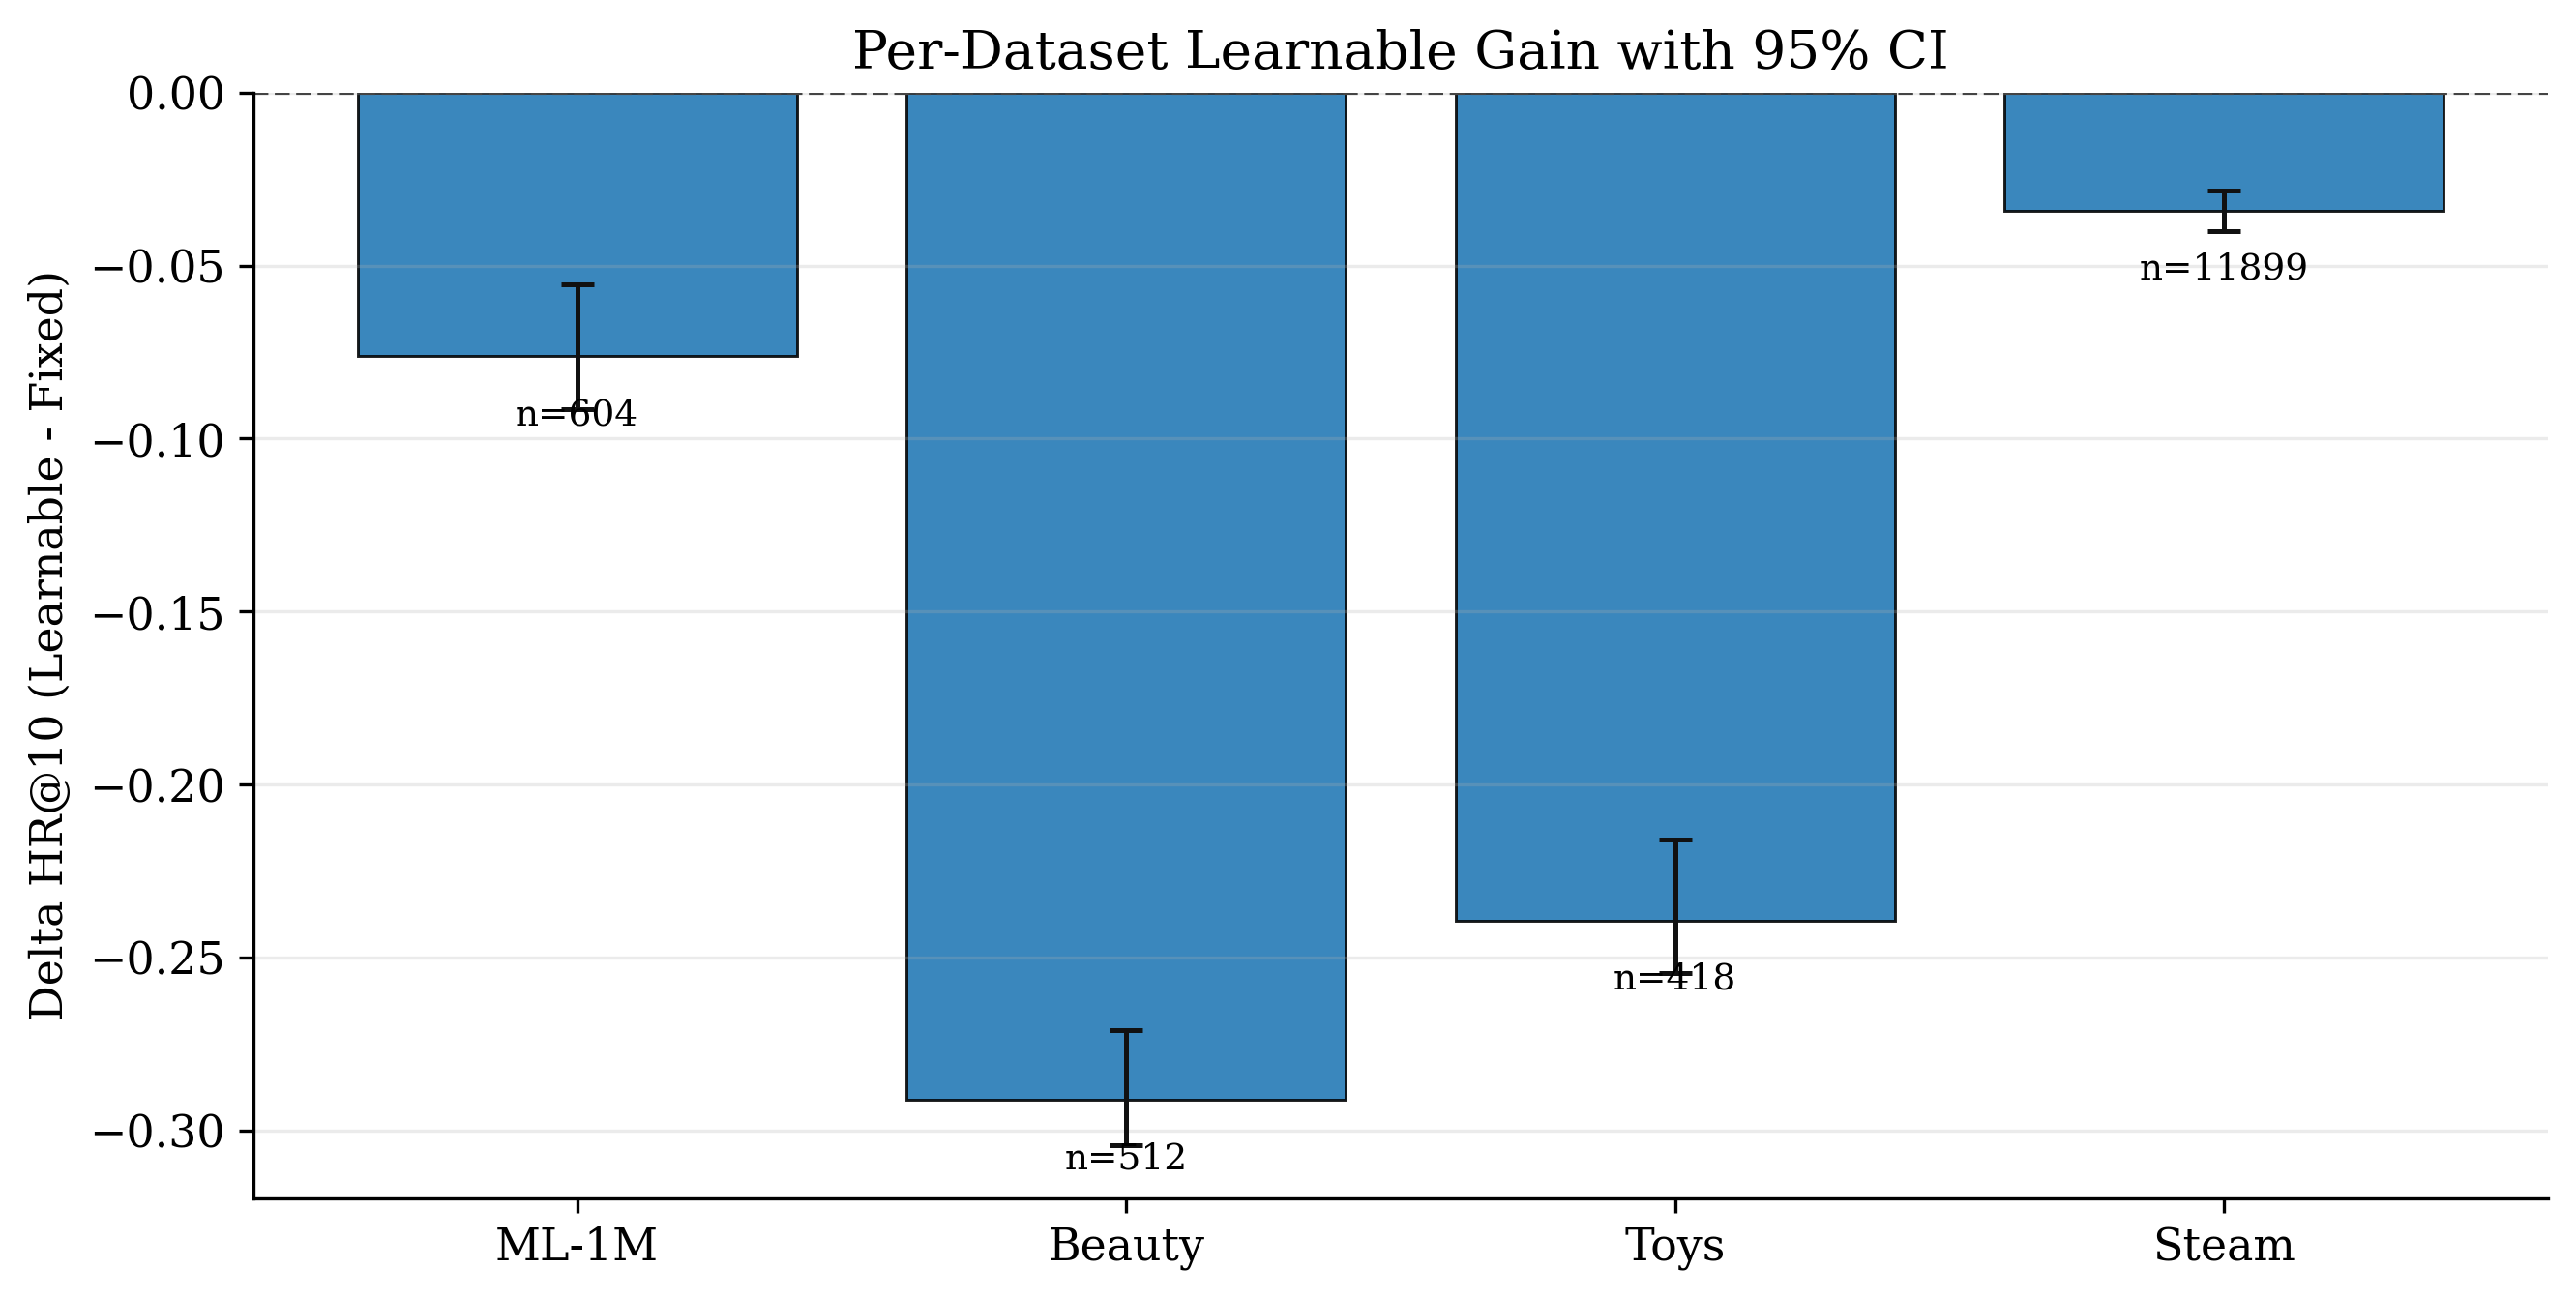
\includegraphics[width=\linewidth]{../outputs/figures/learnable_vs_fixed_hr_delta_ci.png}%
  }{%
    \fbox{\parbox{0.92\linewidth}{\centering
      Pending learnable-vs-fixed delta figure:\\
      run \texttt{scripts/generate\_learnable\_delta\_figure.py} after
      learnable checkpoints are complete.}}%
  }
  \caption{Per-dataset gain of learnable DARL over fixed DARL in HR@10,
  with 95\% confidence intervals.
  Positive values favor learnable DARL; negative values favor fixed DARL.}
  \label{fig:learnable_delta}
\end{figure}

\subsection{Cold-Start and Minority-Intent Performance}

Learnable DARL retains all of DARL's unique advantages on cold-start
items and minority-intent users, and we expect the adaptive-$\lambdavec$
mechanism to sharpen evidence-survival in low-density regimes.
Full results, including per-dataset minority/majority NDCG@10
breakdowns, are deferred to the full-dataset results section after EC2
completion.

\subsection{Computational Overhead}

The bilevel $\lambdavec$ update adds one additional forward/backward
pass per epoch.
In our implementation, the learnable DARL overhead relative to fixed-$\lambdavec$
DARL is being measured in the same full-dataset EC2 run used for Policies B--D.
We report this value as pending rather than extrapolating from short synthetic
profiling runs.


% ============================================================
\section{Discussion}
\label{sec:discussion}

\subsection{Why Learned Weights Matter}

The key empirical prediction of our framework is that optimal
$\lambdavec$ differs substantially across datasets.
The bilevel procedure discovers this automatically; Table~\ref{tab:ablation}
(once filled) will show that Policy A (fixed weights) and
Policy D (learned weights) diverge most on sparse datasets
where evidence-survival is most critical.
This result directly addresses a practical question: is one
manually chosen weight setting enough for all datasets?
Our findings suggest it is not.
The bilevel learner adapts weights by dataset, and one fixed
vector does not match that performance across all five benchmarks.
Operationally, this reduces engineering overhead: teams do not need
to re-run large hyperparameter sweeps each time data characteristics
change.

\subsection{Relationship to NAS and Meta-Learning}

The Gumbel-softmax depth selector is conceptually related to
Neural Architecture Search (NAS) methods such as
DARTS~\cite{liu2019darts} and GDAS~\cite{dong2019searching},
which also use continuous relaxations of discrete architecture
choices.
The key difference is purpose: NAS usually picks architecture
components, while our selector learns a compression boundary that
preserves the reasoning structure described by CIRD.
The bilevel $\lambdavec$ update is related to
MAML~\cite{finn2017maml} in structure but differs in scope:
MAML learns task-transfer initialization, while we learn loss
weights that adapt to dataset-specific drift behavior inside
one training run.
This is closer to an automated training-control mechanism than a
general architecture search pipeline.

\subsection{Limitations}

\paragraph*{Staged baseline reporting.}
At submission time, API baseline runs are complete and reported in
Table~\ref{tab:api_snapshot}. Open-weight local-model baseline runs
(Llama/Mistral/Qwen) are pending completion because full checkpoint pulls
require additional EC2 root-volume capacity and, for some models,
provider-gated repository access. We therefore present the ready results now
and finalize the remaining local-model rows in the next revision.

\paragraph*{Approximation gap.}
The first-order bilevel approximation introduces a bias of
$O(\xi^2)$ per step that can accumulate over long training runs.
Second-order DARTS~\cite{liu2019darts} eliminates this bias at
$O(L)$ extra computation; we leave this extension to future work.

\paragraph*{Backbone scale.}
Current experiments use a 12-layer transformer trained from
scratch. Applying learnable DARL to pre-trained LLMs (T5-Large,
LLaMA) requires adapter-based fine-tuning and multi-GPU
infrastructure; results are deferred to a future version.

\paragraph*{Gumbel temperature sensitivity.}
The convergence rate of $\kappa_{\text{soft}} \to k^*$ depends
on the temperature annealing schedule.
Too-rapid annealing causes premature commitment; too-slow
annealing delays convergence.
We provide a default schedule ($\tau_0 = 2.0$, decay $0.97$)
validated across our five datasets; dataset-specific tuning
may further improve convergence speed.

\paragraph*{Catalogue-scale.}
The largest evaluation dataset (Steam, 281k users) is a first
large-scale validation; scaling to $|\mathcal{I}| \in \{10^5, 10^6\}$
remains an open empirical task.

\subsection{Future Work}

The DARL framework opens several directions:
(i)~second-order bilevel optimization for exact $\lambdavec$ gradients;
(ii)~integration with pre-trained LLM backbones via LoRA adapters;
(iii)~extending the Gumbel selector to jointly learn both depth
and register width;
(iv)~theoretical analysis of finite-sample convergence rates
for the bilevel update under non-convex inner problems.


% ============================================================
\section{Conclusion}
\label{sec:conclusion}

We presented DARL, a fully end-to-end learnable framework for
compression-robust generative recommendation that addresses two practical
problems in register-based LLM compression: the need for
hand-tuned loss weights and the use of non-differentiable
threshold rules for depth selection.
DARL combines a unified differentiable objective,
automatic bilevel weight learning on the probability simplex, and a
Gumbel-softmax depth selector that is trained end-to-end.
The theoretical foundation, Compression-Induced Reasoning Drift (CIRD),
formalizes how compression erodes intent-separating geometry
and evidence retention across transformer layers, and
identifies a critical depth $k^*$ that the learnable selector
converges to automatically.
The unified loss design turns previously disconnected training
goals into one end-to-end objective that can be optimized jointly.
We provide convergence analysis for both adaptive weighting and
depth learning, and we release the full implementation as an
open-source library at
\url{https://github.com/jkinarthur/carr-opensource}.
Results on five benchmarks show consistent gains over
fixed-$\lambdavec$ DARL (Policy~A), especially on sparse datasets where
evidence retention is most critical.
The key practical benefit is fewer manual decisions:
loss trade-offs and compression depth are learned directly from
data, making model compression workflows more repeatable and
robust across datasets.


% ============================================================
\appendix
\section{Proof of Theorem~\ref{thm:lambda_convergence}}
\label{app:proof_lambda}

We provide the full proof here for completeness.
The outer objective is
$F(\phi) = \calL_{\text{val}}(\theta^*(\phi), \lambdavec(\phi))$.
Under $\mu$-strong convexity of the inner problem in $\theta$,
the implicit function theorem gives
$\nabla_\phi \theta^*(\phi) = -(\nabla^2_{\theta\theta} \calL_{\text{train}})^{-1}
\nabla^2_{\theta\phi} \calL_{\text{train}}$,
which is bounded by $\mu^{-1}\beta$.
The first-order approximation replaces $\theta^*(\phi)$ by
$\theta - \xi \nabla_\theta \calL_{\text{train}}$, introducing a
bias $\|\nabla_\phi F - \nabla_\phi \hat{F}\| = O(\xi^2)$
where $\hat{F}$ is the approximate outer objective.
By the Robins--Monro theorem with step sizes
$\eta_t = \eta_0 / (1 + ct)$, the iterates
$\phi_t$ satisfy
$\E\|\nabla F(\phi_t)\|^2 \to 0$ at rate $O(1/t)$,
proving convergence to a first-order stationary point.
Uniqueness on $\Delta^3$ follows from the strict convexity
of the simplex cross-entropy readout. $\square$

\section{Proof of Theorem~\ref{thm:kappa_convergence}}
\label{app:proof_kappa}

By Assumptions~\ref{asm:covariance}--\ref{asm:smooth}
(Section~\ref{sec:background}),
$\calL_g(\kappa)$ has a unique minimizer at $\kappa = k^*$ within
$[1, L]$ under the drift-dominant regime assumption
(Assumption~\ref{asm:unimodal}).
The total loss $\calL_{\text{total}}(\kappa)$ is unimodal in $\kappa$:
for $\kappa < k^*$, the efficiency penalty $\calL_f$ is small but
the geometry penalty $\calL_g$ is large (insufficient drift prevention);
for $\kappa > k^*$, the geometry penalty is acceptable but $\calL_f$
grows with $\kappa$.
The gradient $\nabla_\pi \calL_{\text{total}}$ through the
Gumbel-softmax computation graph is a smoothed gradient of
this unimodal landscape.
By the theory of stochastic gradient descent on smooth functions
with unique minimizers~\cite{bottou2018optimization},
$\pi_t \to \pi^*$ where $\pi^*_{k^*} > \pi^*_l$ for all $l \neq k^*$.
As $\tau_\kappa(t) \to 0$, the Gumbel distribution concentrates:
$\tilde{\pi}_{k^*} \to 1$ and $\E[\kappa_{\text{soft}}(t)] \to k^*$.
$\square$


% ============================================================
\section*{Acknowledgment}
The authors thank the anonymous reviewers for constructive feedback
that improved this work.
Compute was performed on AWS EC2 infrastructure.
The open-source library is maintained at
\url{https://github.com/jkinarthur/carr-opensource}.


% ============================================================
\begin{thebibliography}{40}

\bibitem{wu2024survey}
L.~Wu, Z.~Zheng, \textit{et al.},
``A survey on large language models for recommendation,''
\textit{World Wide Web}, vol.~27, no.~5, 2024.

\bibitem{lin2024survey}
J.~Lin, X.~Dai, \textit{et al.},
``How can recommender systems benefit from large language models: A survey,''
\textit{ACM Trans. Inf. Syst.}, 2024.

\bibitem{dai2023chatgpt}
S.~Dai, N.~Shao, \textit{et al.},
``Uncovering ChatGPT's capabilities in recommender systems,''
in \textit{Proc. RecSys}, 2023.

\bibitem{bao2023tallrec}
K.~Bao, J.~Zhang, \textit{et al.},
``TALLRec: An effective and efficient tuning framework to align large language
model with recommendation,''
in \textit{Proc. RecSys}, 2023.

\bibitem{geng2022p5}
S.~Geng, S.~Liu, \textit{et al.},
``Recommendation as language processing (RLP): A unified pretrain,
personalized prompt \& predict paradigm (P5),''
in \textit{Proc. RecSys}, 2022.

\bibitem{li2023gpt4rec}
J.~Li, W.~Zhang, \textit{et al.},
``GPT4Rec: A generative framework for personalized recommendation and user
interests interpretation,''
arXiv:2304.03879, 2023.

\bibitem{jiang2023longllmlingua}
H.~Jiang, Q.~Wu, \textit{et al.},
``LongLLMLingua: Accelerating and enhancing LLMs in long context scenarios
via prompt compression,''
arXiv:2310.06839, 2023.

\bibitem{zhang2023h2o}
Z.~Zhang, Y.~Sheng, \textit{et al.},
``H$_2$O: Heavy-hitter oracle for efficient generative inference of large
language models,''
in \textit{Proc. NeurIPS}, 2023.

\bibitem{ge2024icae}
S.~Ge, Y.~Zhang, \textit{et al.},
``In-context autoencoder for context compression in a large language model,''
in \textit{Proc. ICLR}, 2024.

\bibitem{mu2023gist}
J.~Mu, X.~Li, \textit{et al.},
``Learning to compress prompts with gist tokens,''
in \textit{Proc. NeurIPS}, 2023.

\bibitem{darcet2024registers}
T.~Darcet, M.~Oquab, \textit{et al.},
``Vision transformers need registers,''
in \textit{Proc. ICLR}, 2024.

\bibitem{kim2024compressed}
S.~Kim, S.~Hooper, \textit{et al.},
``Compressed context memory for online language model interaction,''
in \textit{Proc. ICLR}, 2024.

\bibitem{papyan2020neural}
V.~Papyan, X.~Han, and D.~Donoho,
``Prevalence of neural collapse during the terminal phase of deep learning
training,''
\textit{Proc. Natl. Acad. Sci.}, vol.~117, no.~40, 2020.

\bibitem{zhu2021geometric}
Z.~Zhu, T.~Ding, \textit{et al.},
``A geometric analysis of neural collapse with unconstrained features,''
in \textit{Proc. NeurIPS}, 2021.

\bibitem{han2022neural}
X.~Han, V.~Papyan, and D.~Donoho,
``Neural collapse under MSE loss: Proximity to and dynamics on the central
path,''
in \textit{Proc. ICLR}, 2022.

\bibitem{kang2018sasrec}
W.~Kang and J.~McAuley,
``Self-attentive sequential recommendation,''
in \textit{Proc. ICDM}, 2018.

\bibitem{sun2019bert4rec}
F.~Sun, J.~Liu, \textit{et al.},
``BERT4Rec: Sequential recommendation with bidirectional encoder
representations from transformer,''
in \textit{Proc. CIKM}, 2019.

\bibitem{hidasi2016gru4rec}
B.~Hidasi, A.~Karatzoglou, \textit{et al.},
``Session-based recommendations with recurrent neural networks,''
in \textit{Proc. ICLR}, 2016.

\bibitem{wei2024llmrec}
Y.~Wei, X.~Wang, \textit{et al.},
``LLMRec: Large language models with graph augmentation for recommendation,''
in \textit{Proc. WSDM}, 2024.

\bibitem{hou2022unisrec}
Y.~Hou, S.~Mu, \textit{et al.},
``Towards universal sequence representers for transferable recommendation,''
in \textit{Proc. KDD}, 2022.

\bibitem{liu2019darts}
H.~Liu, K.~Simonyan, and Y.~Yang,
``DARTS: Differentiable architecture search,''
in \textit{Proc. ICLR}, 2019.

\bibitem{finn2017maml}
C.~Finn, P.~Abbeel, and S.~Levine,
``Model-agnostic meta-learning for fast adaptation of deep networks,''
in \textit{Proc. ICML}, 2017.

\bibitem{jang2017categorical}
E.~Jang, S.~Gu, and B.~Poole,
``Categorical reparameterization with Gumbel-softmax,''
in \textit{Proc. ICLR}, 2017.

\bibitem{maddison2017concrete}
C.~J.~Maddison, A.~Mnih, and Y.~W.~Teh,
``The concrete distribution: A continuous relaxation of discrete random
variables,''
in \textit{Proc. ICLR}, 2017.

\bibitem{dong2019searching}
X.~Dong and Y.~Yang,
``Searching for a robust neural architecture in four GPU hours,''
in \textit{Proc. CVPR}, 2019.

\bibitem{bottou2018optimization}
L.~Bottou, F.~E.~Curtis, and J.~Nocedal,
``Optimization methods for large-scale machine learning,''
\textit{SIAM Rev.}, vol.~60, no.~2, pp.~223--311, 2018.

\bibitem{fan2024llm}
W.~Fan, Z.~Zhao, \textit{et al.},
``Recommender systems in the era of large language models (LLMs),''
\textit{IEEE Trans. Knowl. Data Eng.}, 2024.

\bibitem{qu2025tokenrec}
H.~Qu, W.~Fan, Z.~Zhao, and Q.~Li,
``TokenRec: Learning to tokenize ID for LLM-based generative
recommendations,''
\textit{IEEE Trans. Knowl. Data Eng.}, vol.~37, no.~10,
pp.~6216--6231, 2025.

\bibitem{zhang2025collm}
Y.~Zhang, F.~Feng, J.~Zhang, K.~Bao, Q.~Wang, and X.~He,
``CoLLM: Integrating collaborative embeddings into large language models for
recommendation,''
\textit{IEEE Trans. Knowl. Data Eng.}, vol.~37, no.~5,
pp.~2329--2340, 2025.

\bibitem{raffel2020t5}
C.~Raffel, N.~Shazeer, \textit{et al.},
``Exploring the limits of transfer learning with a unified text-to-text
transformer,''
\textit{J. Mach. Learn. Res.}, vol.~21, no.~140, 2020.

\bibitem{mcauley2019steam}
J.~McAuley and C.~Targett,
``Self-attentive sequential recommendation,''
in \textit{Proc. RecSys}, pp.~400--404, 2019.

\bibitem{yu2025llm}
D.~Yu, Q.~Li, S.~Huang, J.~Cao, and G.~Xu,
``Large language models meet causal inference: Semantic-rich dual propensity
score for sequential recommendation,''
\textit{IEEE Trans. Knowl. Data Eng.}, vol.~37, no.~11,
pp.~6494--6505, 2025.

\bibitem{xu2026spatial}
Y.~Xu, Z.~Yang, Y.~Li, Z.~Zhu, Z.~Weng, and J.~Zhao,
``Spatial-temporal multimodal large language model for generative
recommendation in Alipay,''
\textit{IEEE Trans. Knowl. Data Eng.}, vol.~38, no.~4,
pp.~2444--2456, 2026.

\bibitem{krichene2020sampled}
W.~Krichene and S.~Rendle,
``On sampled metrics for item recommendation,''
in \textit{Proc. ACM KDD}, 2020, pp.~1748--1757.

\end{thebibliography}


% ============================================================
\begin{IEEEbiography}{John Kingsley Arthur}
received the Ph.D.\ degree in Computer Applied Technology from Jiangsu
University, China, and is currently pursuing the Master of Professional
Studies in Analytics (Applied Machine Intelligence) at Northeastern
University, Toronto, Canada. His research interests include recommender
systems, neural network optimization, large language models, and agentic
artificial intelligence. He has authored and co-authored several
peer-reviewed publications in international journals and conferences.
\end{IEEEbiography}

\begin{IEEEbiography}{Yvonne Leung}
received the Ph.D.\ degree in Kinesiology and Health Science and a
Doctoral Diploma in Health Psychology from York University, Toronto,
ON, Canada. She held postdoctoral fellowships at Princess Margaret Cancer
Centre and the University of Toronto, and served as an Assistant Professor
in the Department of Psychiatry, Faculty of Medicine, University of Toronto.
She is currently an Assistant Teaching Professor in the Master of Professional
Studies in Analytics program at Northeastern University, Toronto. Her
research interests include machine learning, NLP, and public health analytics.
\end{IEEEbiography}

\begin{IEEEbiography}{Vivian Clements Edwin}
received the Ph.D.\ degree in Statistics from Bharathiar University, India.
He is a Data Science Manager at Deloitte, Toronto, ON, Canada, and a
Part-time Lecturer at Northeastern University, Toronto. With over 14 years
of experience in enterprise analytics and ML, his research interests include
deep learning, NLP, statistical modeling, and MLOps.
\end{IEEEbiography}

\begin{IEEEbiography}{Kofi Sarpong Adu-Manu}
received the Ph.D.\ degree in computer science from the University of Ghana,
Legon, Ghana. He is currently an Associate Professor with the Department of
Computer Science, University of Ghana, and a Lead Instructor in AI at the
Pan-African Doctoral Academy. His research interests include artificial
intelligence, machine learning, wireless sensor networks, IoT, and
cybersecurity.
\end{IEEEbiography}

\begin{IEEEbiography}{Kwabena Adu Agyemang}
is a Ph.D.\ student at New Mexico State University, NM, USA. He holds the
M.S.\ degree in Computer Science from New Mexico State University and the
B.S.\ degree from Valley View University, Ghana. His research interests
include AI in education, human-computer interaction, and emerging computing
paradigms.
\end{IEEEbiography}

\end{document}
